\scanpage{9}

$\gamma')$ $\forall A,B\in F_0$, l'intersection des $\in F_0$ qui contiennent $A\cap\complement B$ est $\in F_0$ (i.e. il y a un plus petit $C\in F_0$ qui contienne $A\cap\complement B$).

C'est suffisant, car on prend la top. $T$ \deleted{\unsure{formée par}}\inserted{dont les fermés sont} les intersections quelconques d'élts de $F_0$ [ils sont stables par réunions finies, comme on voit tout de suite]. Cette topologie \inserted{est} \deleted{satisfait} visiblement la moins fine parmi celles qu'on envisage. Elle est caractérisée par le fait qu'elle satisfait la condition

\deleted{\unsure{l'ensemble ouvert}} $(*)$ Tout ouvert de $X$ est réunion d'ouverts de $X$ qui sont $\in F$, ou encore tout fermé de $X$ est int. de fermés qui sont $\in F$, ou encore $\deleted{\forall}\unsure{\forall}$ les $x\in X$ a un syst. fond. de voisinages $\in F$ (ou de voisinages ouverts $\in F$) ....

\margin{\deleted{\uline{Condition f} Si $A\in F$ est loc. fermé (donc de la forme $B-C$, $B,C\in F_0$, $C$ non dense $B$) alors \deleted{\unsure{l'ens des}} composantes connexes de $A$ \deleted{\unsure{est}} \inserted{\unsure{sont en nb}} \uuline{\unsure{finies|fini}} (donc \deleted{\unsure{fermées}}\inserted{\unsure{ouvertes}}) et sont $\in F_0$.}}

\uline{NB} Supposons que $F$ satisfasse a)b)c)d), \unsure{je dis que|pr dire que} \deleted{\illegible{2}} si $A\in F$, alors $\dot A$ \inserted{\figure{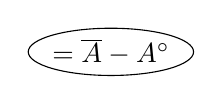
\begin{tikzpicture}[baseline=-0.6ex]\draw (0,0) ellipse (1.05 and .3);\node at (0,0) {$=\overline A-A^\circ$};\end{tikzpicture}}} est \uline{rare} dans $X$, \deleted{En effet, $\dot A=\overline A-A^\circ$, et $A^\circ$, i.e. $\dot A$} l'intérieur \inserted{$U$} de $\dot A$ est vide. On sait que $U\in F$, \unsure{nous restreignons nous à} $U$ [cela conserve a)b)c)d)] on est ramené à prouver que si $\overline A=X$, $A^\circ=\varnothing$, alors $\deleted{\unsure{X|A}}=\varnothing$. \inserted{\unsure{on utilise par d)} $A^\circ$ \unsure{est} dense dans $\deleted{X}=\overline A$ ...}

\mspage{10}
